\documentclass[border=10pt]{standalone}
\usepackage{tkz-fct}
\usepackage{tkz-base}
\usepackage{array}
\usepackage{amsmath}
\begin{document}

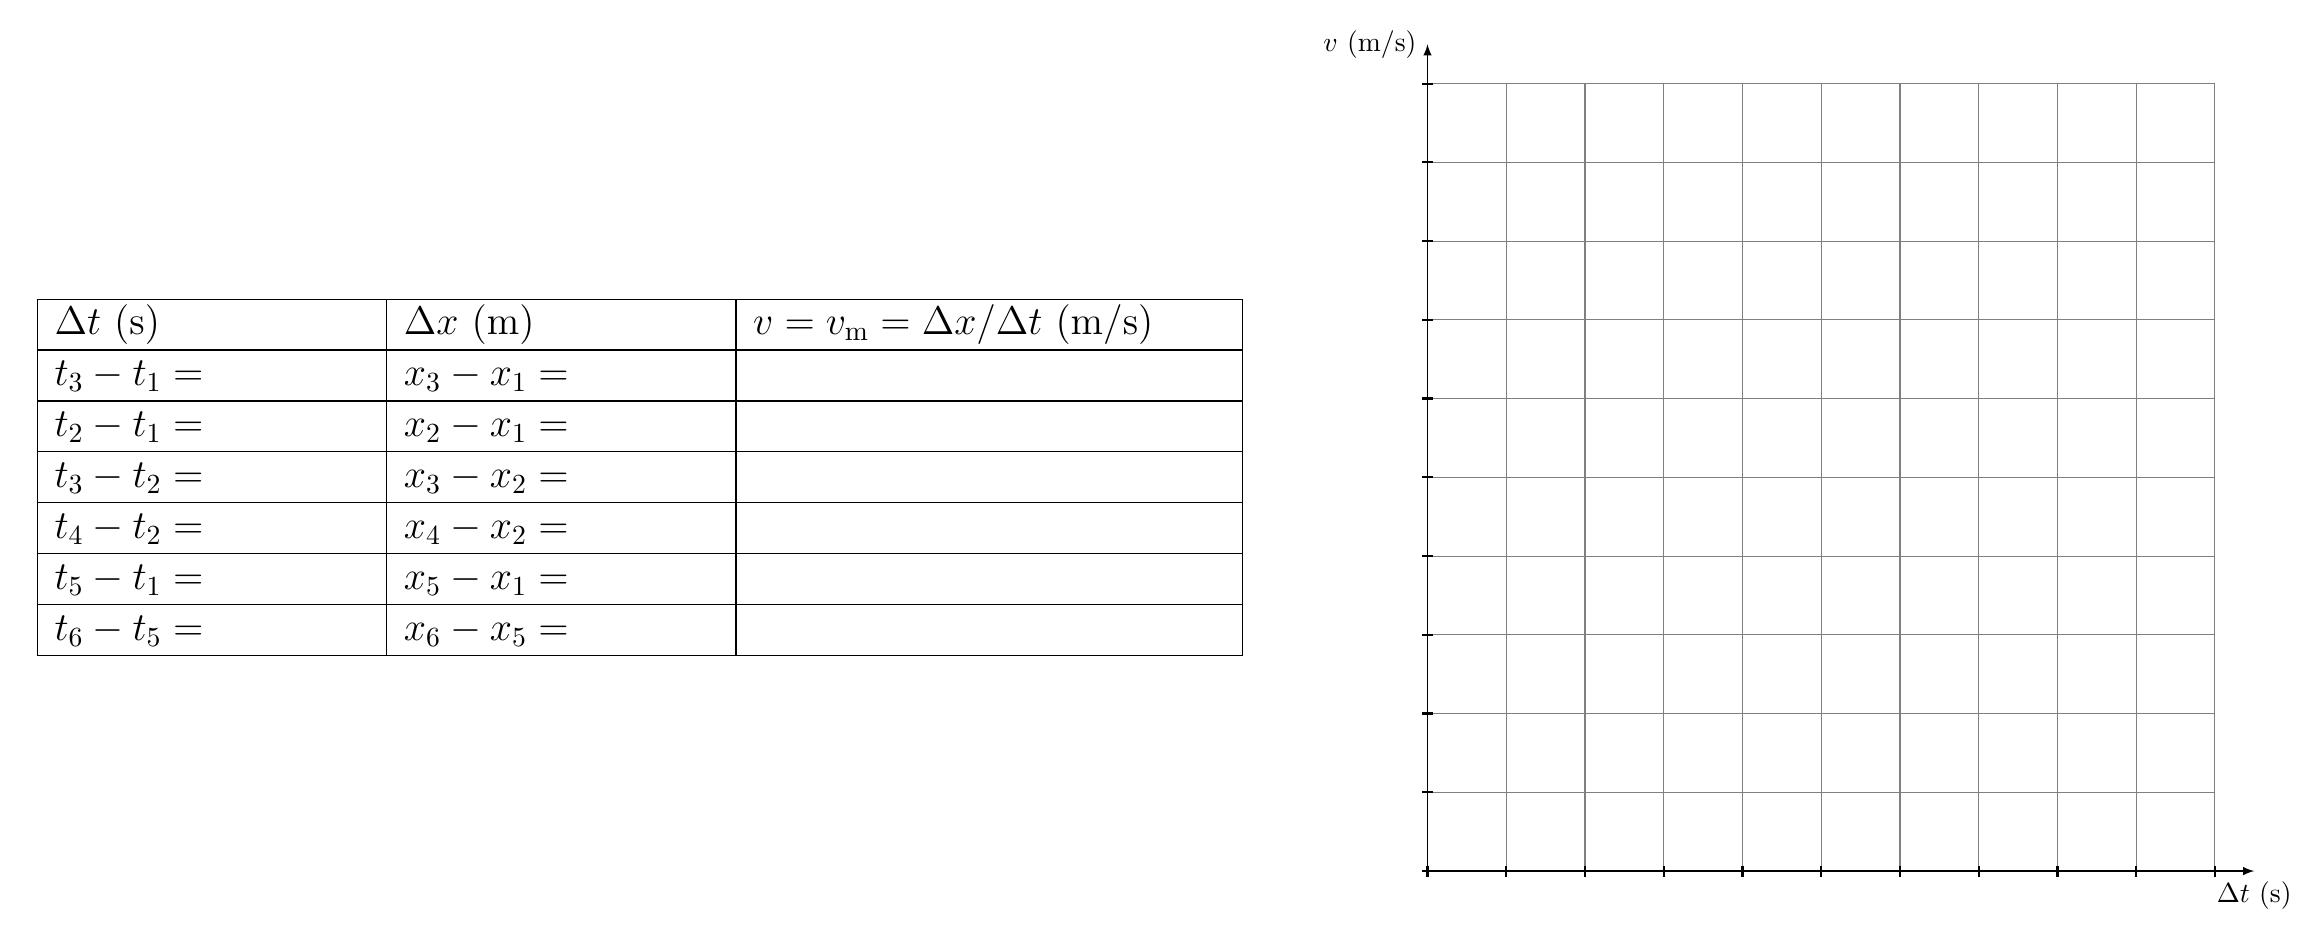
\begin{tikzpicture}
% Tableau en LaTeX standard avec tkz-text
\tkzText(-10,5){\Large
    \begin{tabular}{|p{4cm}|p{4cm}|p{6cm}|}
        \hline
        $\Delta t$ (s)& $\Delta x$ (m) & $v=v_{\text{m}}=\Delta x/\Delta t$ (m/s) \\
        \hline
        $t_{3}-t_{1}=$&$x_{3}-x_{1}=$& \\
        \hline
        $t_{2}-t_{1}=$&$x_{2}-x_{1}=$& \\
        \hline
        $t_{3}-t_{2}=$&$x_{3}-x_{2}=$& \\
        \hline
        $t_{4}-t_{2}=$&$x_{4}-x_{2}=$& \\
        \hline
        $t_{5}-t_{1}=$&$x_{5}-x_{1}=$& \\
        \hline
       $t_{6}-t_{5}=$ &$x_{6}-x_{5}=$ & \\
        \hline
    \end{tabular}
}

% Repère quadrillé
\begin{scope}[yscale=1]
\tkzInit[xmin=0,xmax=10,ymin=0,ymax=20, ystep=2]
\tkzGrid
\tkzDrawX[label = $\Delta t$ (s)]
\tkzDrawY[label = $v$ (m/s)]

\end{scope}
\end{tikzpicture}

\end{document}
